\documentclass{osa-article}
\journal{osac}
\usepackage{subcaption}
\begin{document}
\title{Lensless Image Classification for Machine-based Decision Making}

\author{Brian Rodriguez,\authormark{1} Ganghun Kim,\authormark{1,2} and Rajesh Menon\authormark{1,*}}

\address{\authormark{1}Department of Electrical and Computer Engineering, University of Utah, Salt Lake City, UT 84112}
\address{\authormark{1}Currently with Apple Inc, Cupertino CA}

\email{\authormark{*}remenon@eng.utah.edu} %% email address is required

\begin{abstract}
Deep Learning (DL) has accelerated advancements in Image Classification via convolutional neural networks (CNNs). However, these image classification tasks have been widely trained on images taken with typical cameras; human-centric images. Here, we present a CNN trained using data taken by a bare CMOS image sensor with no lens. We created a dataset of lensless images comprised of handwritten digits taken from the MNIST dataset. Then, we trained a CNN on this dataset and were able to show that for 10 digits, the CNN is able to classify lensless images with 97\% accuracy.
\end{abstract}
%
\section{Introduction}
Wide-scale deep learning algorithms have pushed image classification tasks to their limits. State of the art architectures have been able to classify human-centric images with astonishing accuracy, but human-centric images require expensive cameras \cite{DBLP:journals/corr/SimonyanZ14a, DBLP:journals/corr/SzegedyIV16}. Recently, lensless imaging has been gaining traction \cite{DBLP:journals/corr/AsifASVB15, Gill:13, DBLP:journals/corr/KimIPM17}. These lensless images are taken using a low cost and light-weight image sensor without the use of a camera lens. Previously, we demonstrated that machine learning algorithms can accurately classify lensless images for 2 digits with 99\% accuracy using support vector machines (SVMs) \cite{DBLP:journals/corr/abs-1709-00408}. Here, we extend this idea and use DL to accurately classify lensless images for 10 digits. Moreover, we trained a CNN on a dataset of lensless images that we captured using a lensless camera.
%
\begin{figure}[!ht]
\centering
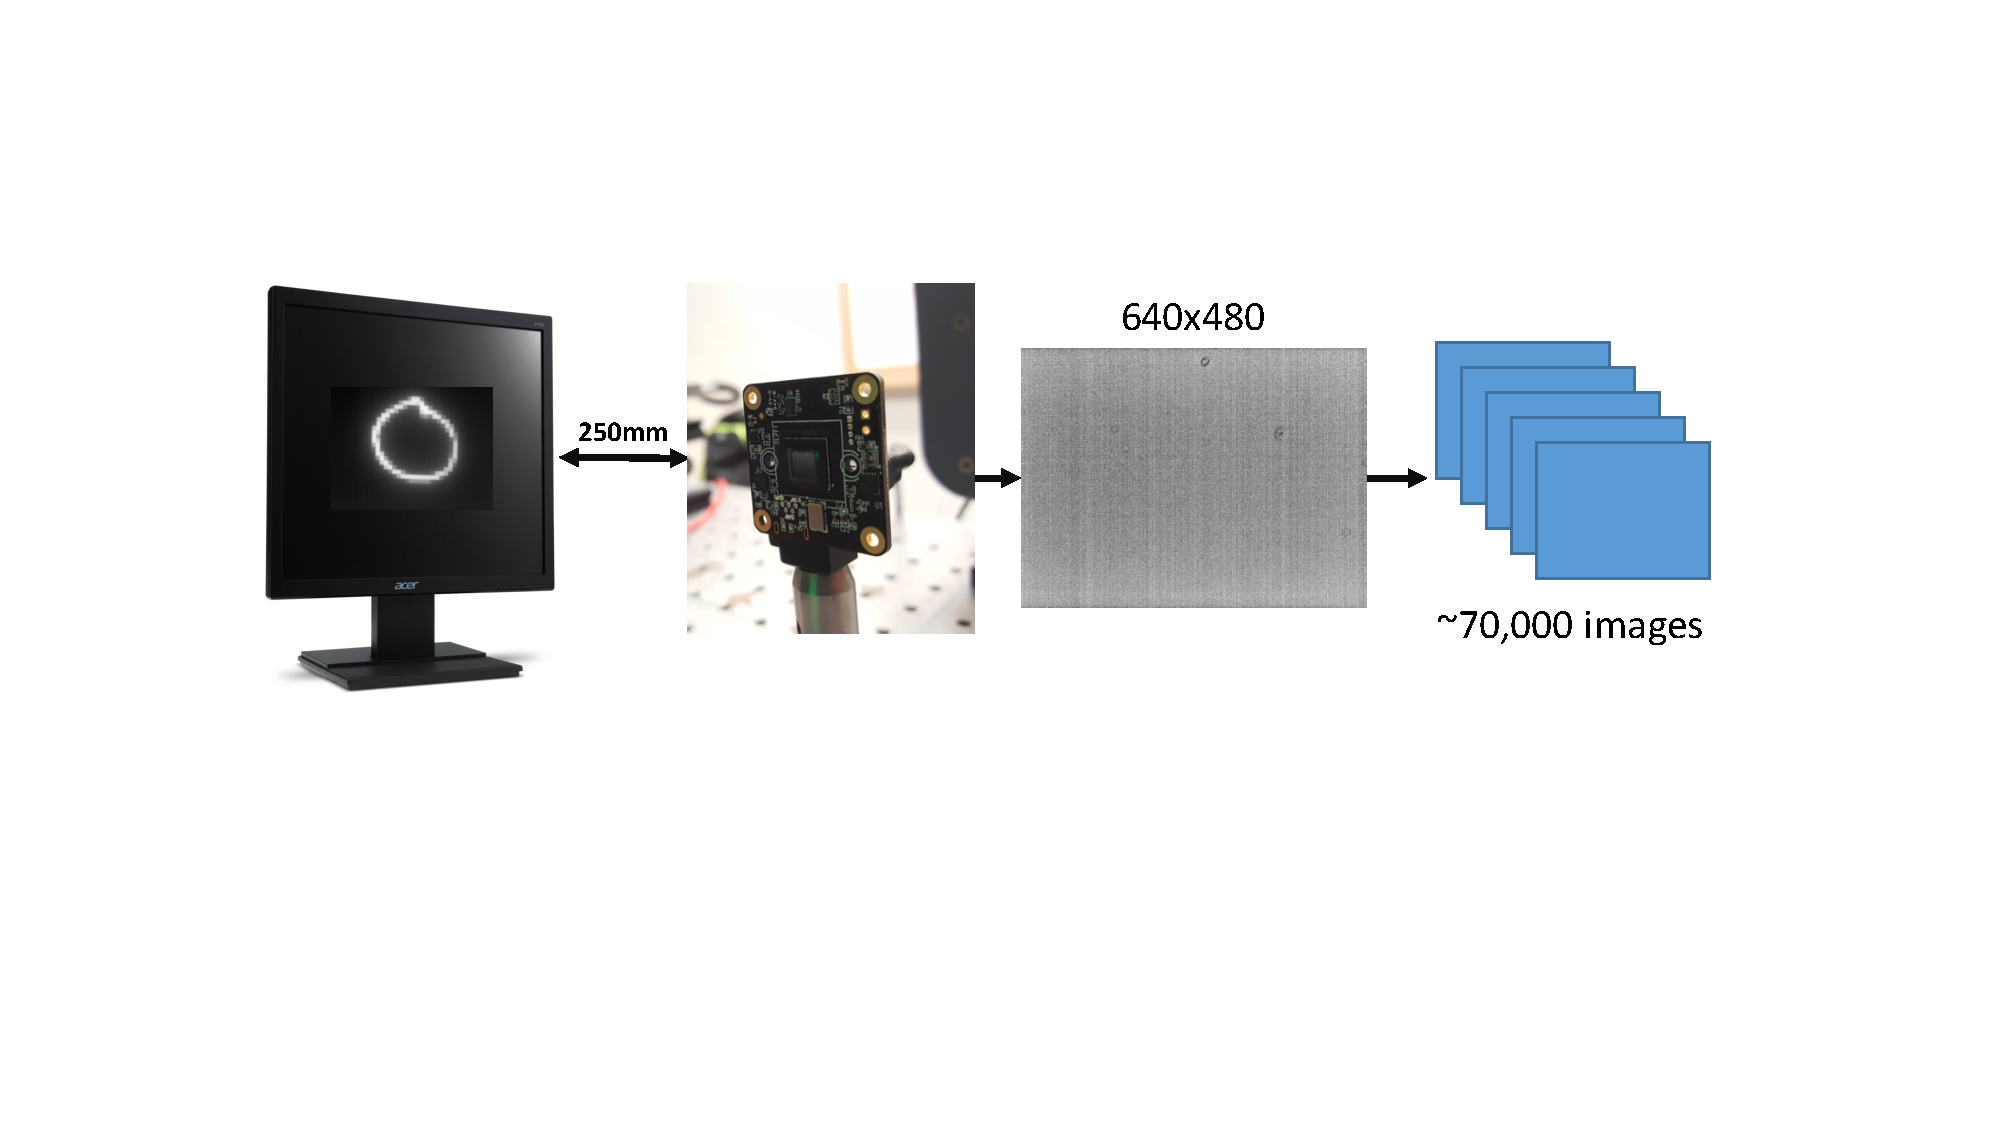
\includegraphics[width=1\linewidth]{imagingprocess}
\caption{Lensless imaging process from left to right. The process begins with an LCD screen that displays an image of a digit then the image sensor captures an image of the screen. These images are collected into a dataset and used as input for the neural network.}\label{imagingprocess}
\end{figure}
%
Our lensless camera consists of a bare CMOS image sensor. We used a liquid-crystal display (LCD) that displayed images of hand-written digits taken from the open-sourced MNIST dataset \cite{lecun-mnisthandwrittendigit-2010}. The LCD rests 250mm away from the CMOS sensor with an exposure time of 150ms and averaged over 100 frames to reduce noise. In contrast to other ``lensless'' imagers, which typically include amplitude or phase masks, our camera has no optics in front of the sensor at all. Using this procedure, we captured 70,000 lensless images and created a dataset with appropriate labels. These lensless images are 640x480 (307,200 pixels per image) which for scalability purposes are resized to 240x240.
%
Our results demonstrate that CNNs can accurately classify multiple classes of data taken directly from a lensless camera.
%
\section{Background}
Convolutional neural networks are widely used for object recognition, computer vision, and image classification tasks. Recent advancements such as YOLOv3, a real-time object detection network, and Inception-v4, a large-scale image classification network, have set high expectations for proceeding networks \cite{DBLP:journals/corr/abs-1804-02767, DBLP:journals/corr/SzegedyIV16}. While these networks occupy different subfields in DL, most convolutional neural networks use the same operations to perform classification. Ideas such as convolution, pooling, and activation functions are the cores of a convolutional neural network. \par
Convolution (Conv) is an operation that takes in an input image or filter and performs a dot product within the scope of its receptive field, which corresponds to a scalar point on an output feature map (filter) as shown in Figure \ref{conv}. A receptive field is the area in which the convolution operation performs its dot product on. In Figure \ref{conv}, the receptive field is a 3x3 area as denoted by the white 3x3 box. After it does a dot product on the first section, the receptive field slides to the right and performs another dot product until it reaches the end of the image.\par
Since convolution is a linear operation, using an activation function allows a neural network to learn nonlinear relations in data. In this paper we utilize the widely used Rectified Linear Unit activation function (ReLU) \cite{Nair:2010:RLU:3104322.3104425}. The ReLU activation function is represented as $f(x) = max(0, x) $ where \textit{x} is a neuron in the neural network. Maxpooling is a type of pooling operation, which is more notably used for nonlinearly down-sampling its input. Depending on the receptive field size of the pooling operation, it takes a max filter over the receptive field and takes the highest value in that field as shown in Figure \ref{pool}. \par
After various feature extracting layers (conv and pooling layers), it is typical to see either one or two fully-connected layers (FC) at the end of a network. An FC layer is what a CNN utilizes to make high-level predictions based on the data. Every neuron in an FC layer is connected to all of the previous layer's activations allowing the network to ``see'' what high-level features the convolution layers extracted from the data. These FC layers take input from pooling layers and ``squash'' or squeeze this input from a 3-dimensional array into a 1-dimensional array. This allows for the FC layer to connect to all of parameters from the pooling layer to its own neurons as shown in Figure \ref{fc_layer}.\par
\begin{figure}[!ht]
\centering
\begin{subfigure}[b]{0.5\textwidth}
   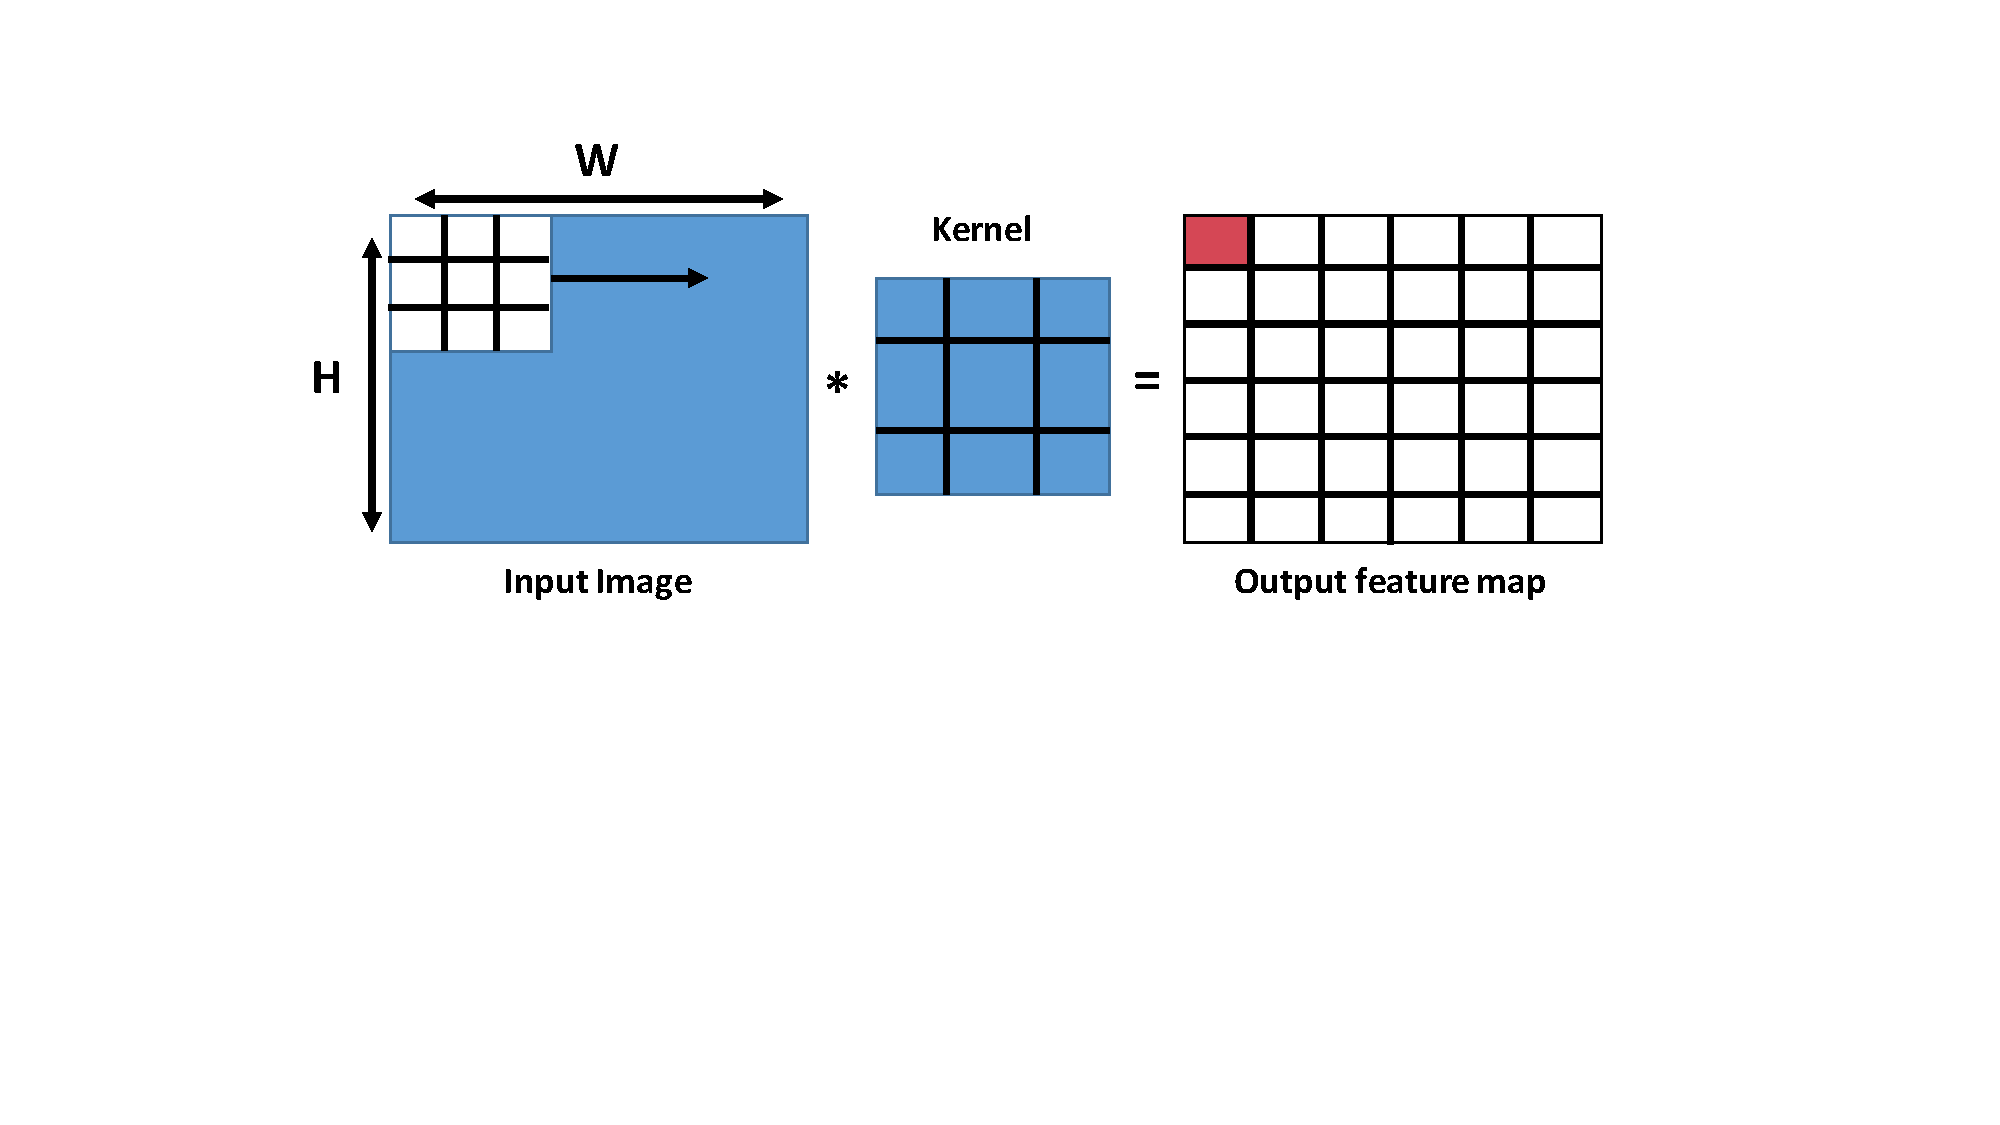
\includegraphics[width=1\linewidth]{convolution}
   \caption{}
   \label{conv} 
\end{subfigure}\hfill
\begin{subfigure}[b]{0.45\textwidth}
   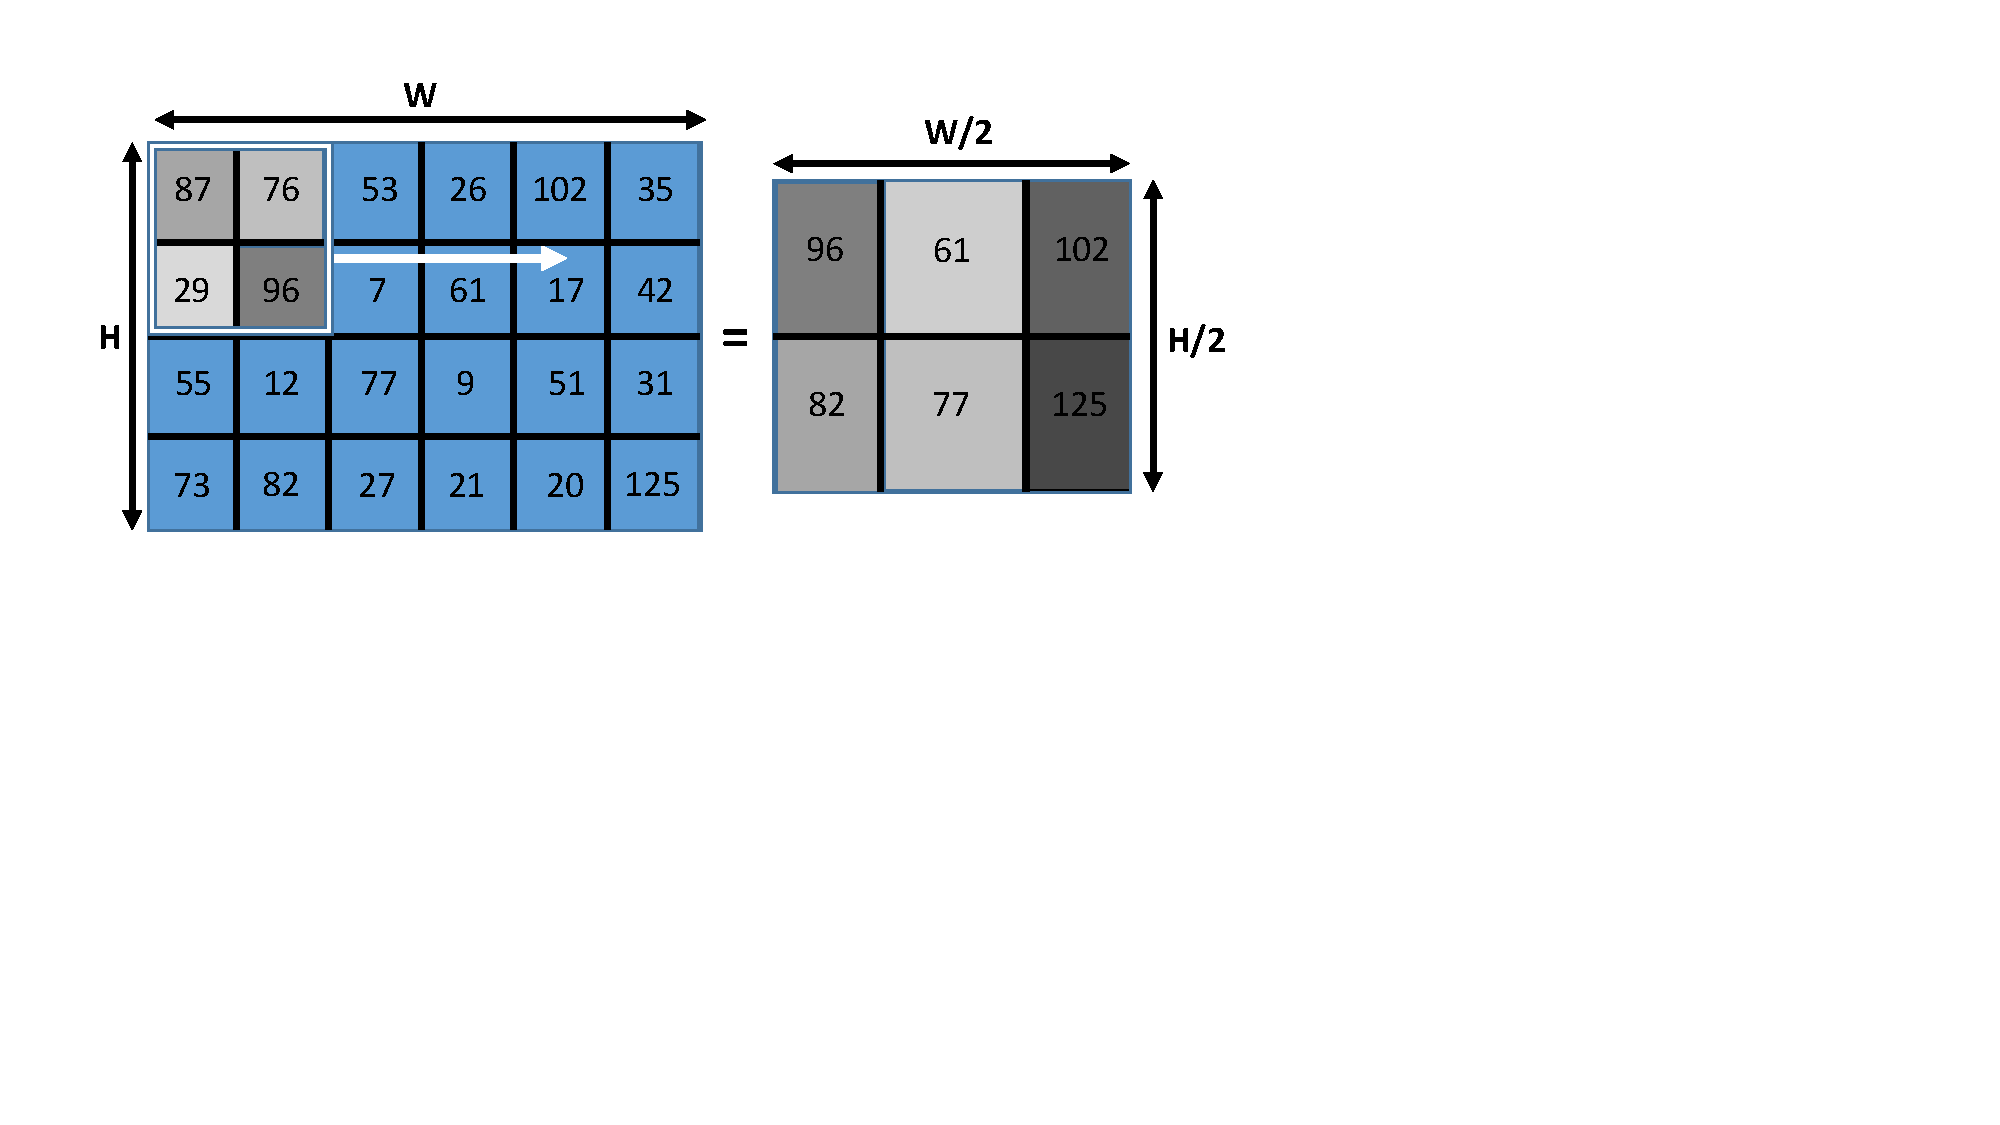
\includegraphics[width=1\linewidth]{maxpool}
   \caption{}
   \label{pool}
\end{subfigure}
\caption{(a) Example of the convolution operation with a 3x3 receptive field where one stride to the right corresponds to one scalar output on the feature map (filter). (b) An example of a maxpooling operation. In this example, we use a 2x2 receptive field and a stride of 2 to down-sample the image in half.}\label{conv_max_operations}
%(b) Shows the graph of the ReLU activation function. The function takes the max of either 0 or \textit{x} where x is a neuron in the network. This is important because this means that the neuron is either on or off.
\end{figure}
Other important concepts regarding neural networks are back-propagation, mini-batch size and learning rate. Back-propagation is the backbone of how a neural network is able to learn \cite{Rumelhart:1988:LRB:65669.104451}. Back-propagation is a type of gradient-descent optimization algorithm that propagates an error value calculated using a loss function. It takes this error value and computes the partial derivative with respect to a parameter value to calculate the gradients of all the parameters in the network. This allows the network to learn values for all of its parameters to achieve a global minimum that will make the error value the smallest. \par
A mini-batch size is the amount of data inputs a neural network will ``see'' before it computes an error value. This allows the network to learn in small incremental steps, rather than learning over an entire dataset. Learning rates impact parameter updates. The bigger the learning rate the more a parameter will change, but the lower the learning rate the less a parameter will be impacted by an update from back-propagation.
\begin{figure}[!ht]
\centering
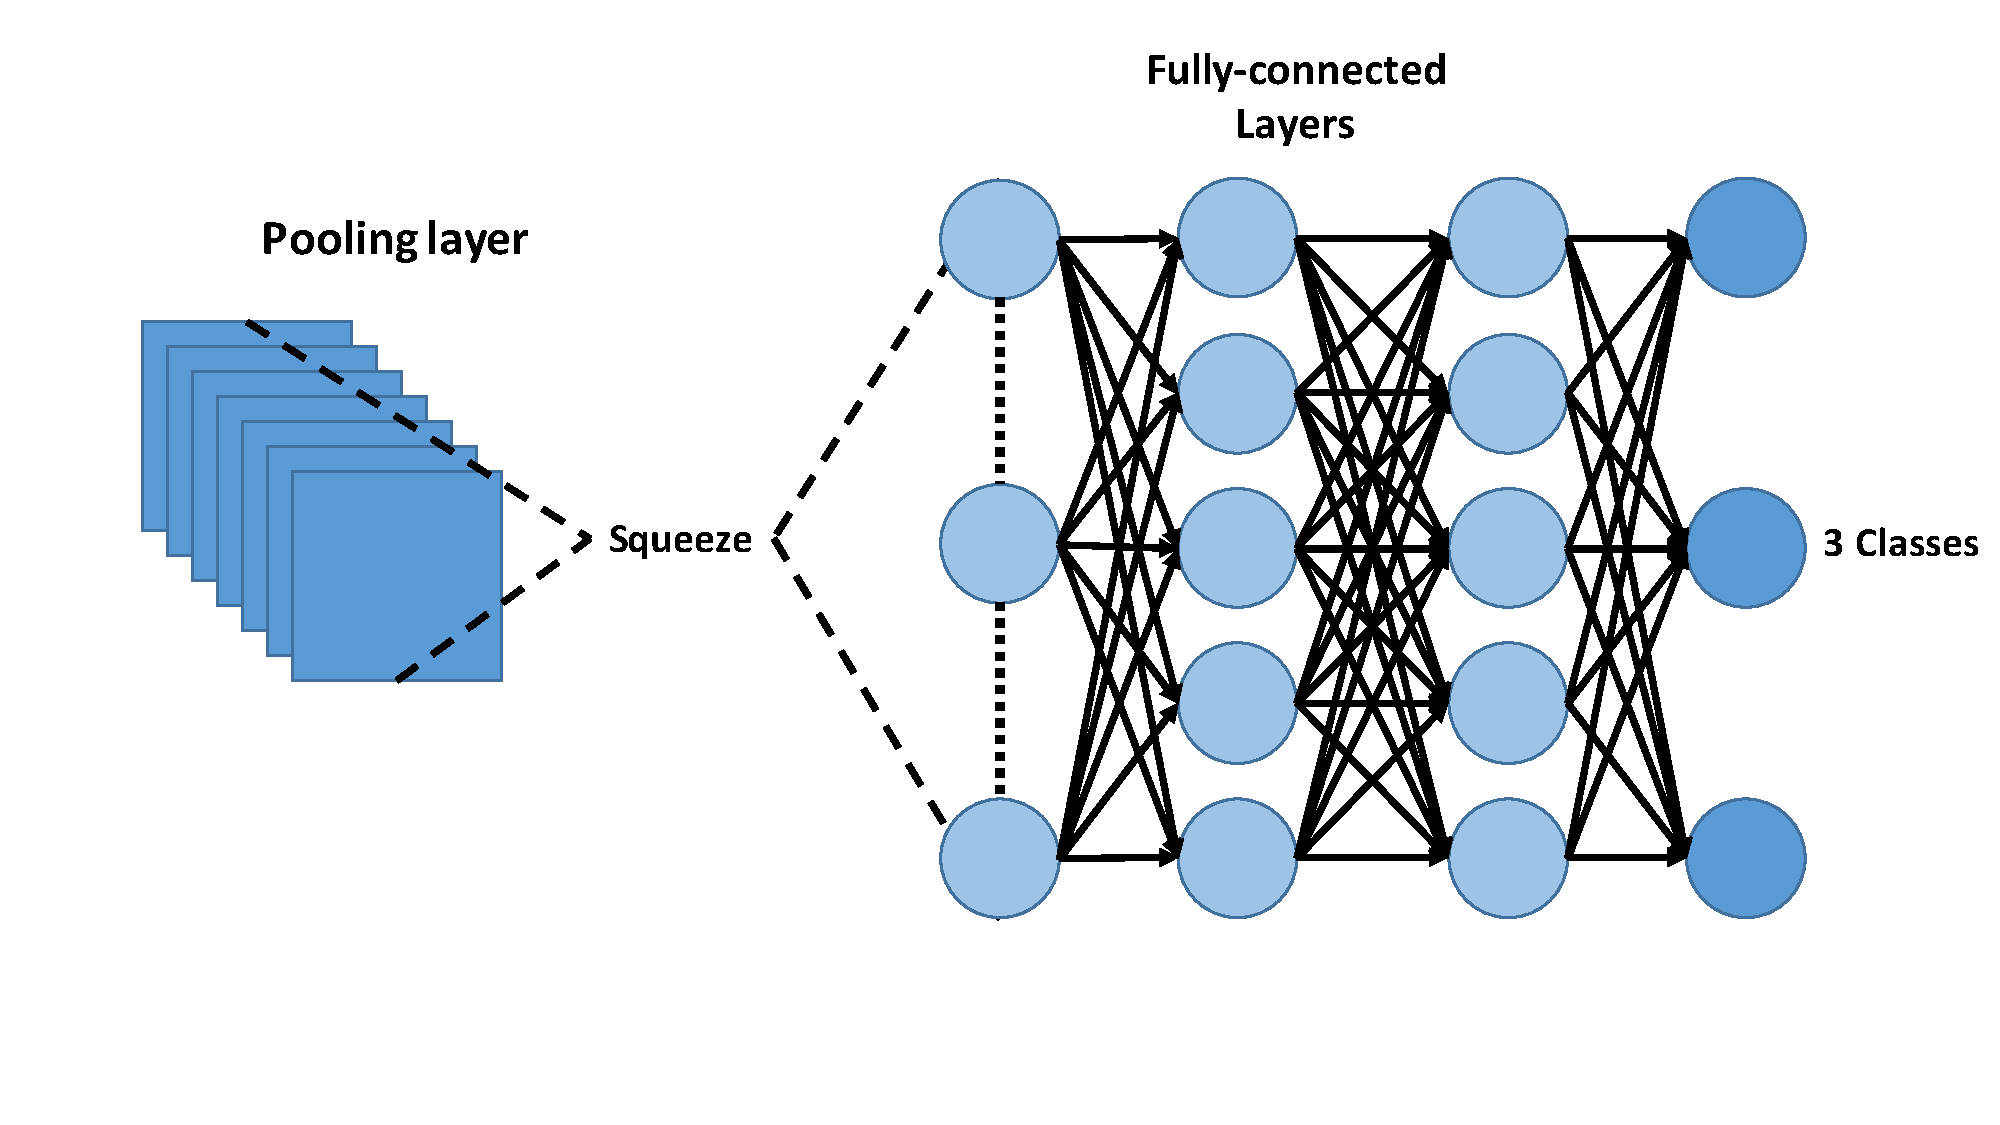
\includegraphics[width=1\linewidth]{fc}
\caption{Example of a fully-connected layer. All of the connections in the previous layer are connected to the next layer's neurons, in this case, every filter after a maxpooling layer is ``squashed'' to form a 1-dimensional array of neurons. This 1-dimensional array is then connected to all of the neurons of the FC layer. Following is another FC layer connecting the previous FC layer and 3 arbitrary classes of a dataset. }\label{fc_layer}
\end{figure}
%
\section{Network Architecture}
We propose a CNN architecture that is able to classify lensless images at a 97\% accuracy. Our architecture is comprised of two main sections; feature section and a classifying section. The feature section has 4 subsections containing convolutional layers and max pooling layers. Each convolutional layer is followed by batch normalization and a ReLU activation function \cite{DBLP:journals/corr/IoffeS15, Nair:2010:RLU:3104322.3104425}.
%
 The 1x1 convolutional layers are used for dimensionality reduction, these layers follow every pooling layer except for the last \cite{DBLP:journals/corr/LinCY13}. The 1x1 convolutions allowed for our network to converge faster. \par
Following the feature section is a classifying section. This section contains two fully-connected layers, where the last fully-connected layer classifies between the 10 different classes shown in Figure \ref{classifying}. After the fully-connected layers is a softmax function that compresses the output scores of the CNN into values ranging from 0 to 1 where all of the values sum up to 1. This is important in multi-class classification problems, since the softmax function outputs action probabilities relating to each class  \cite{Bishop:2006:PRM:1162264, Sutton:1998:IRL:551283}. \par
Overfitting is a problem in neural networks that impacts validation accuracy. It's a problem where the neural network memorizes the input data instead of learning the required features to make accurate predictions. To combat this problem we employed dropout on our final fully-connected layer with a probability of .5 \cite{JMLR:v15:srivastava14a}. Dropout is an idea that ``turns off'' or more accurately zeroes out neurons, which forces the network to learn even more connections between a layer.
%
\begin{figure}
  \begin{subfigure}{0.30\textwidth}
    \centering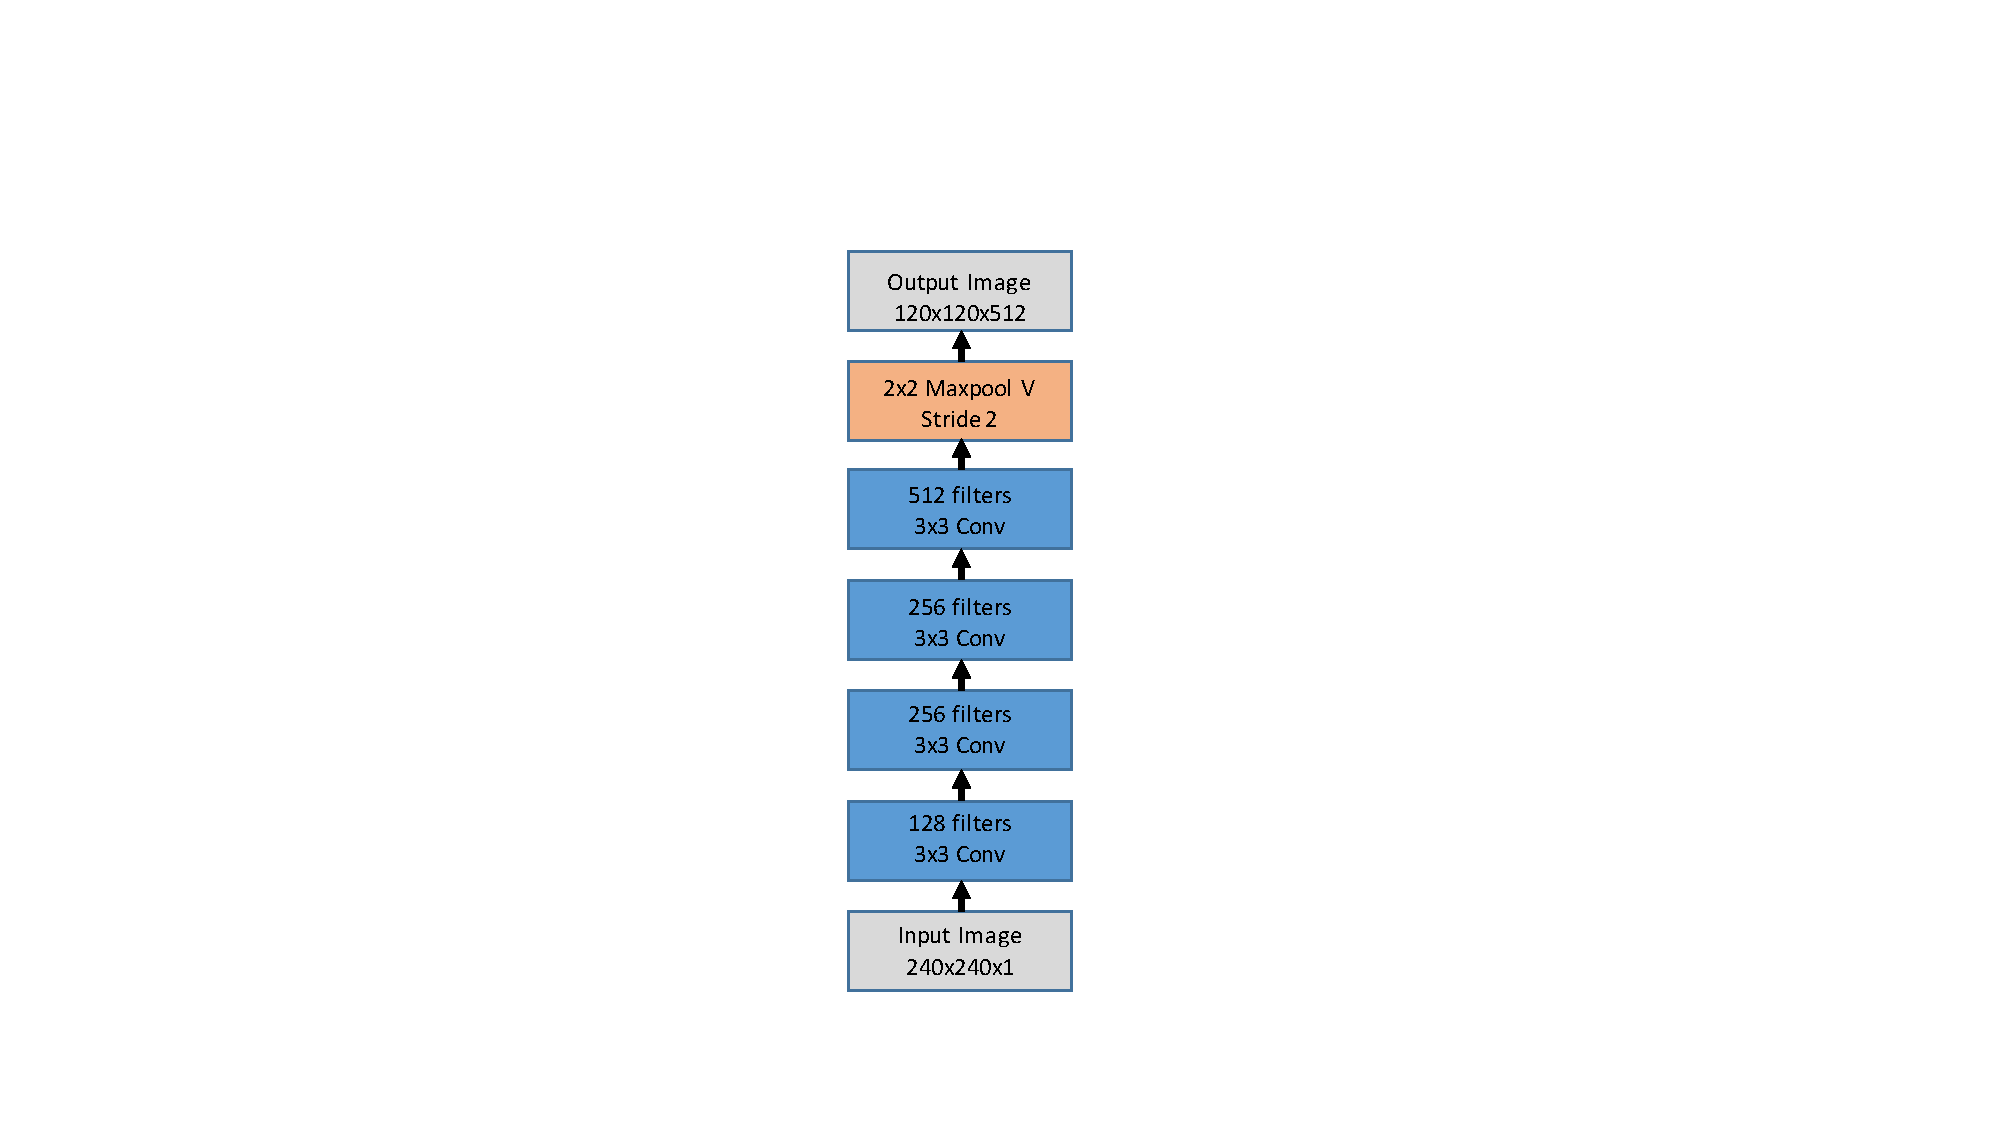
\includegraphics[width=.48\linewidth]{section1}
    \caption{Section 1 of the Convolutional Neural Network. Input images are sized to 240x240 and gray-scaled.}\label{section1}
  \end{subfigure}\hfill
  \begin{subfigure}{0.30\textwidth}
    \centering
    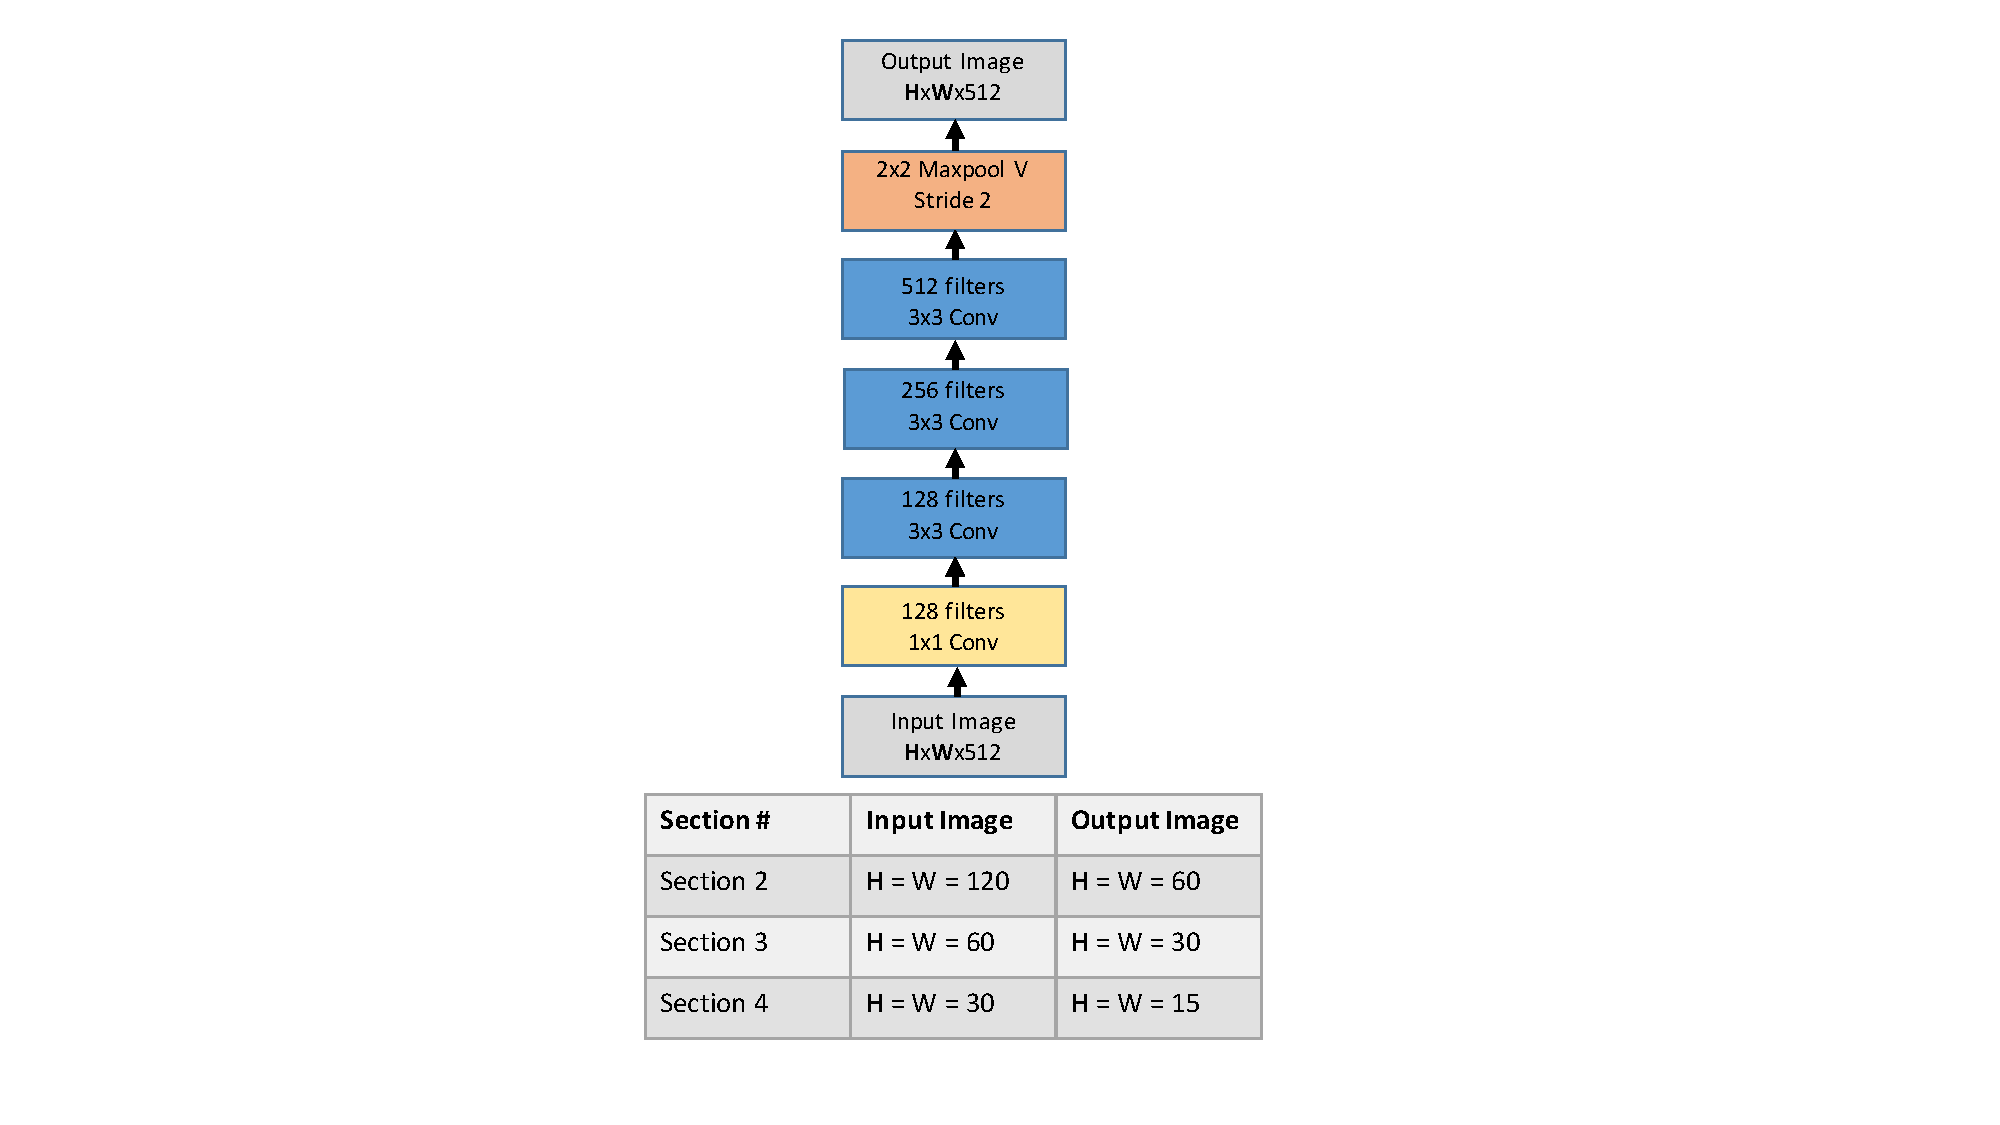
\includegraphics[width=1.1\linewidth]{section_x}
    \caption{Sections 2, 3, and 4 of the network. These sections have the exact same layout but differ with respect to input and output dimensions of the images.}\label{sec_x}
  \end{subfigure}\hfill
  \begin{subfigure}{0.30\textwidth}
    \centering
    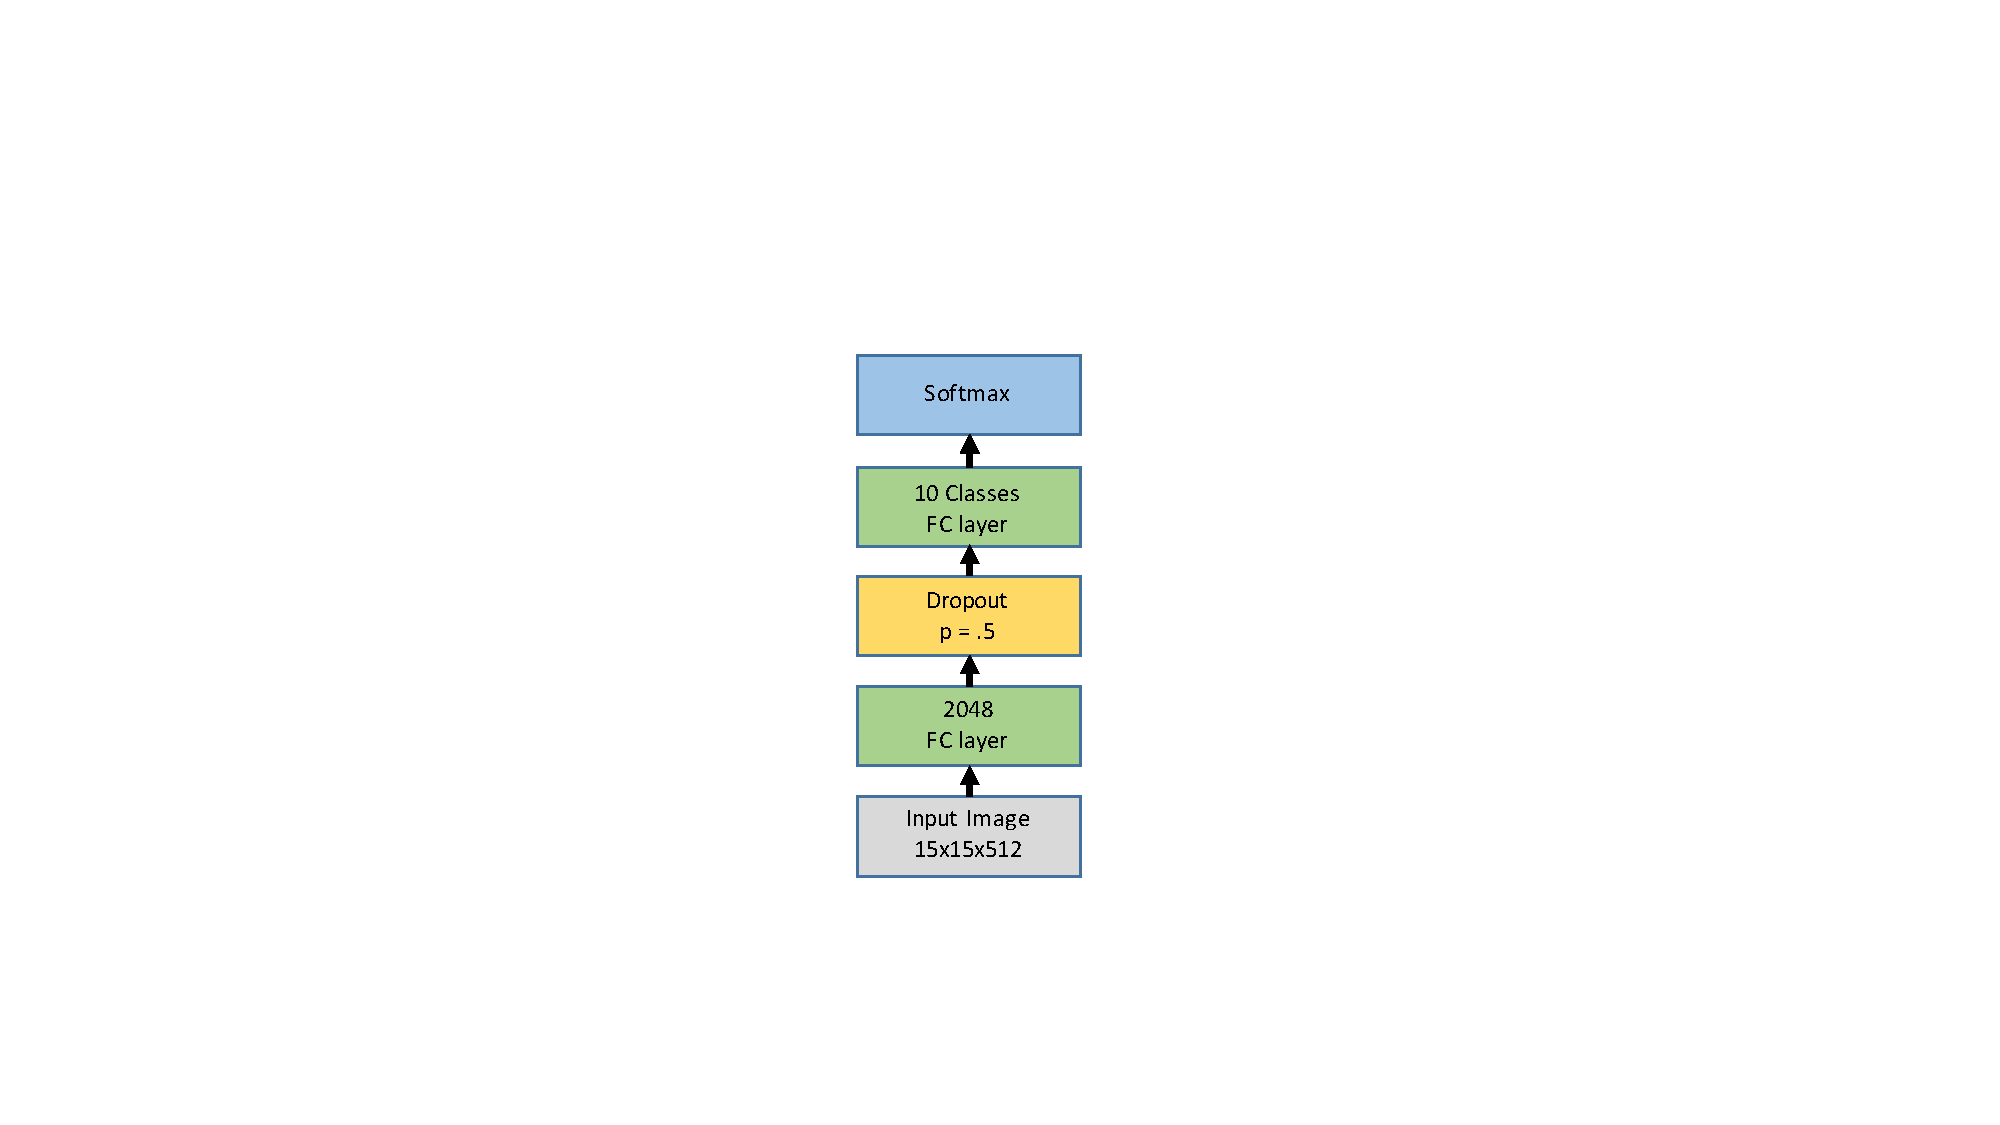
\includegraphics[width=.55\linewidth]{classifying_sec}
    \caption{The classification section of the network.}\label{classifying}
  \end{subfigure}
  \caption{The entire network architecture from (a)-(c) where the input and output images are 3-dimensional. The dimensions represent height, width and channels (filters), respectively.}
\end{figure}
%
\section{Training Methodology}
We created our network using Pytorch, a highly extensible deep learning framework \cite{paszke2017automatic}. Our network was trained using stochastic gradient descent with a momentum of .9 on a single NVidia Tesla V100 GPU \cite{DBLP:journals/corr/KingmaB14, Sutskever:2013:IIM:3042817.3043064}. We used a learning rate of .001 and a mini-batch size of 16. The learning rate was decayed when the loss plateaued; decaying one time over 40 epochs. The input data are gray-scaled (by default) and the images are resized to 240x240. 5,400 images were taken from each class and split into two groups, training and testing groups; 3,200 training images and 2,200 testing images. Testing images are used to benchmark our model and test for overfitting in the network.
%
\begin{figure}[!ht]
\centering
\begin{subfigure}[b]{0.45\textwidth}
   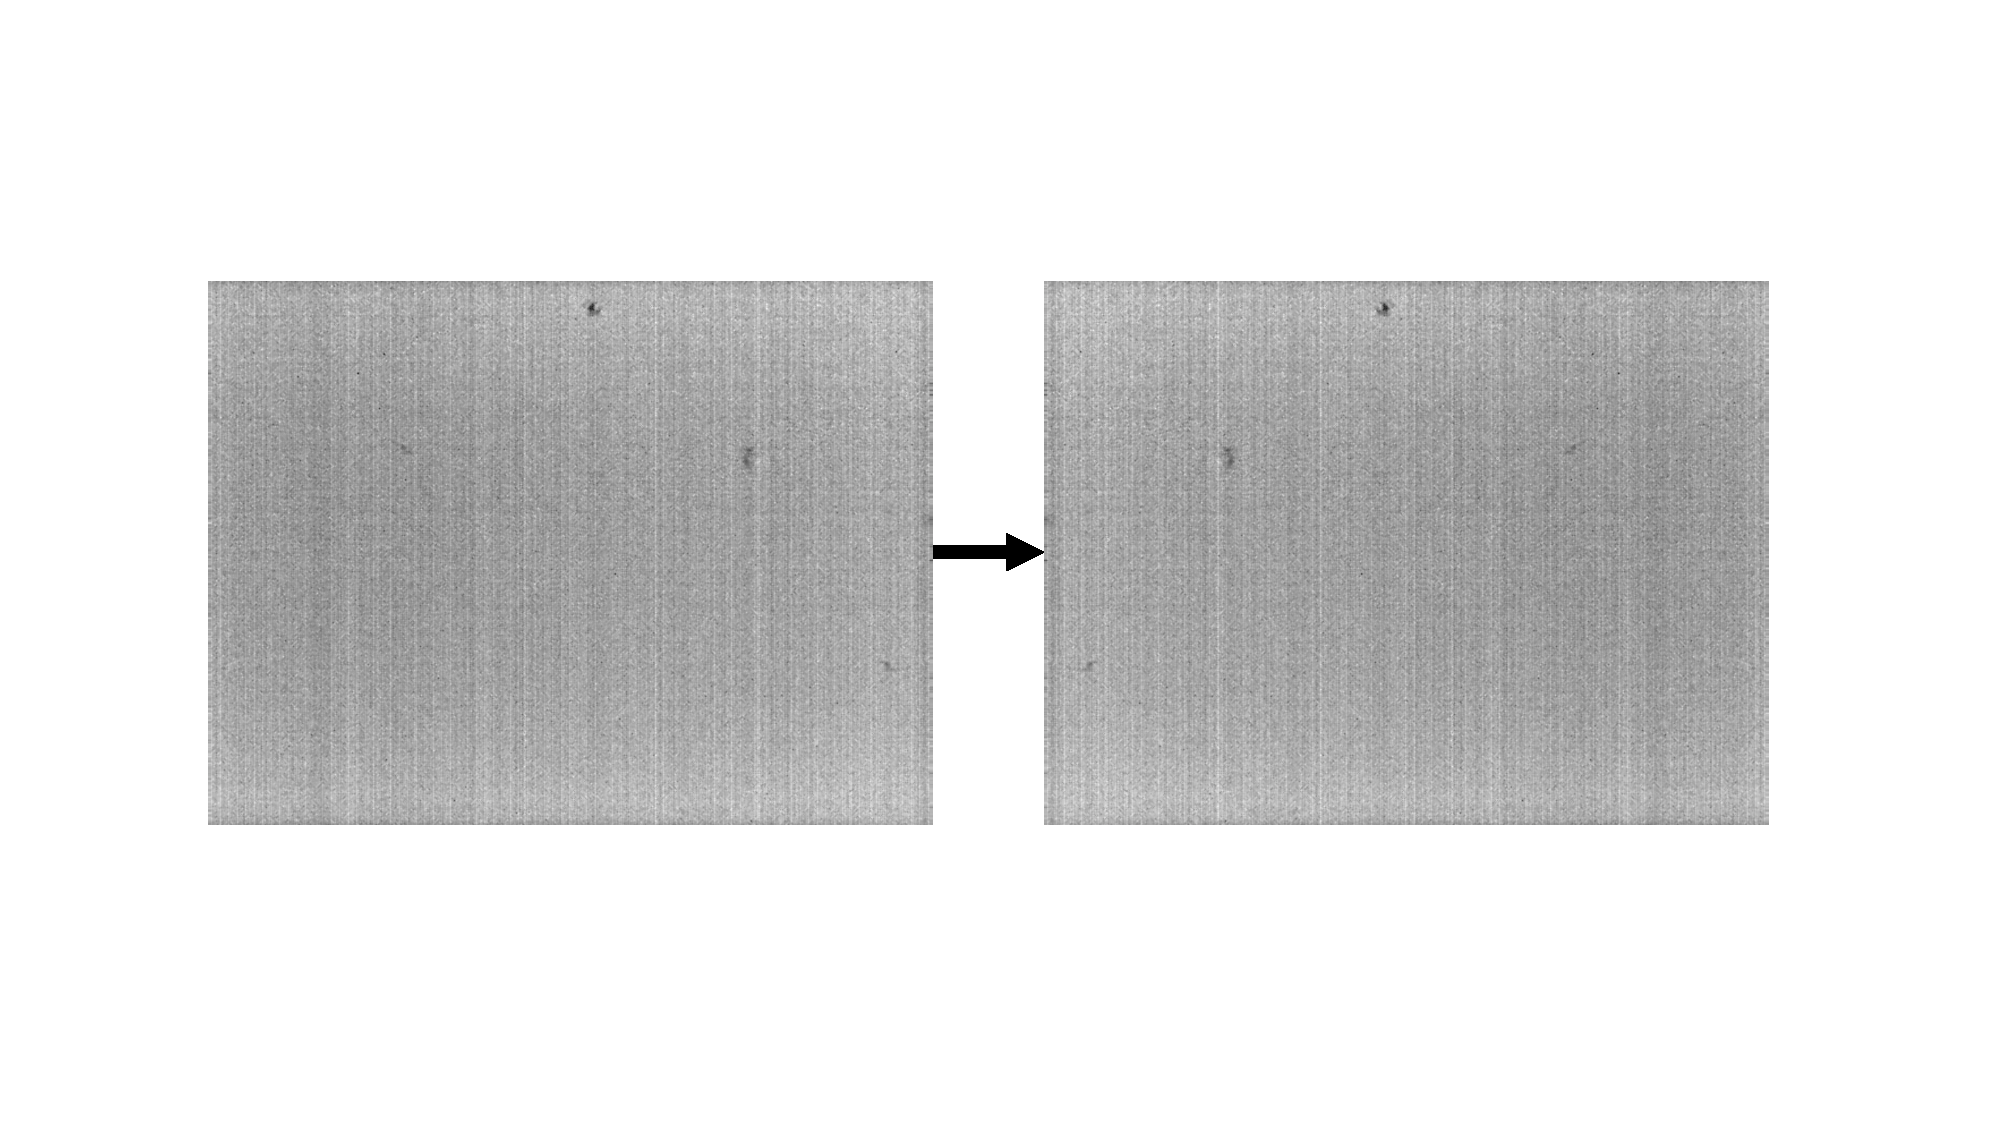
\includegraphics[width=1\linewidth]{lensless_hflip}
   \caption{}
   \label{fig:Ng1} 
\end{subfigure}\hfill
\begin{subfigure}[b]{0.45\textwidth}
   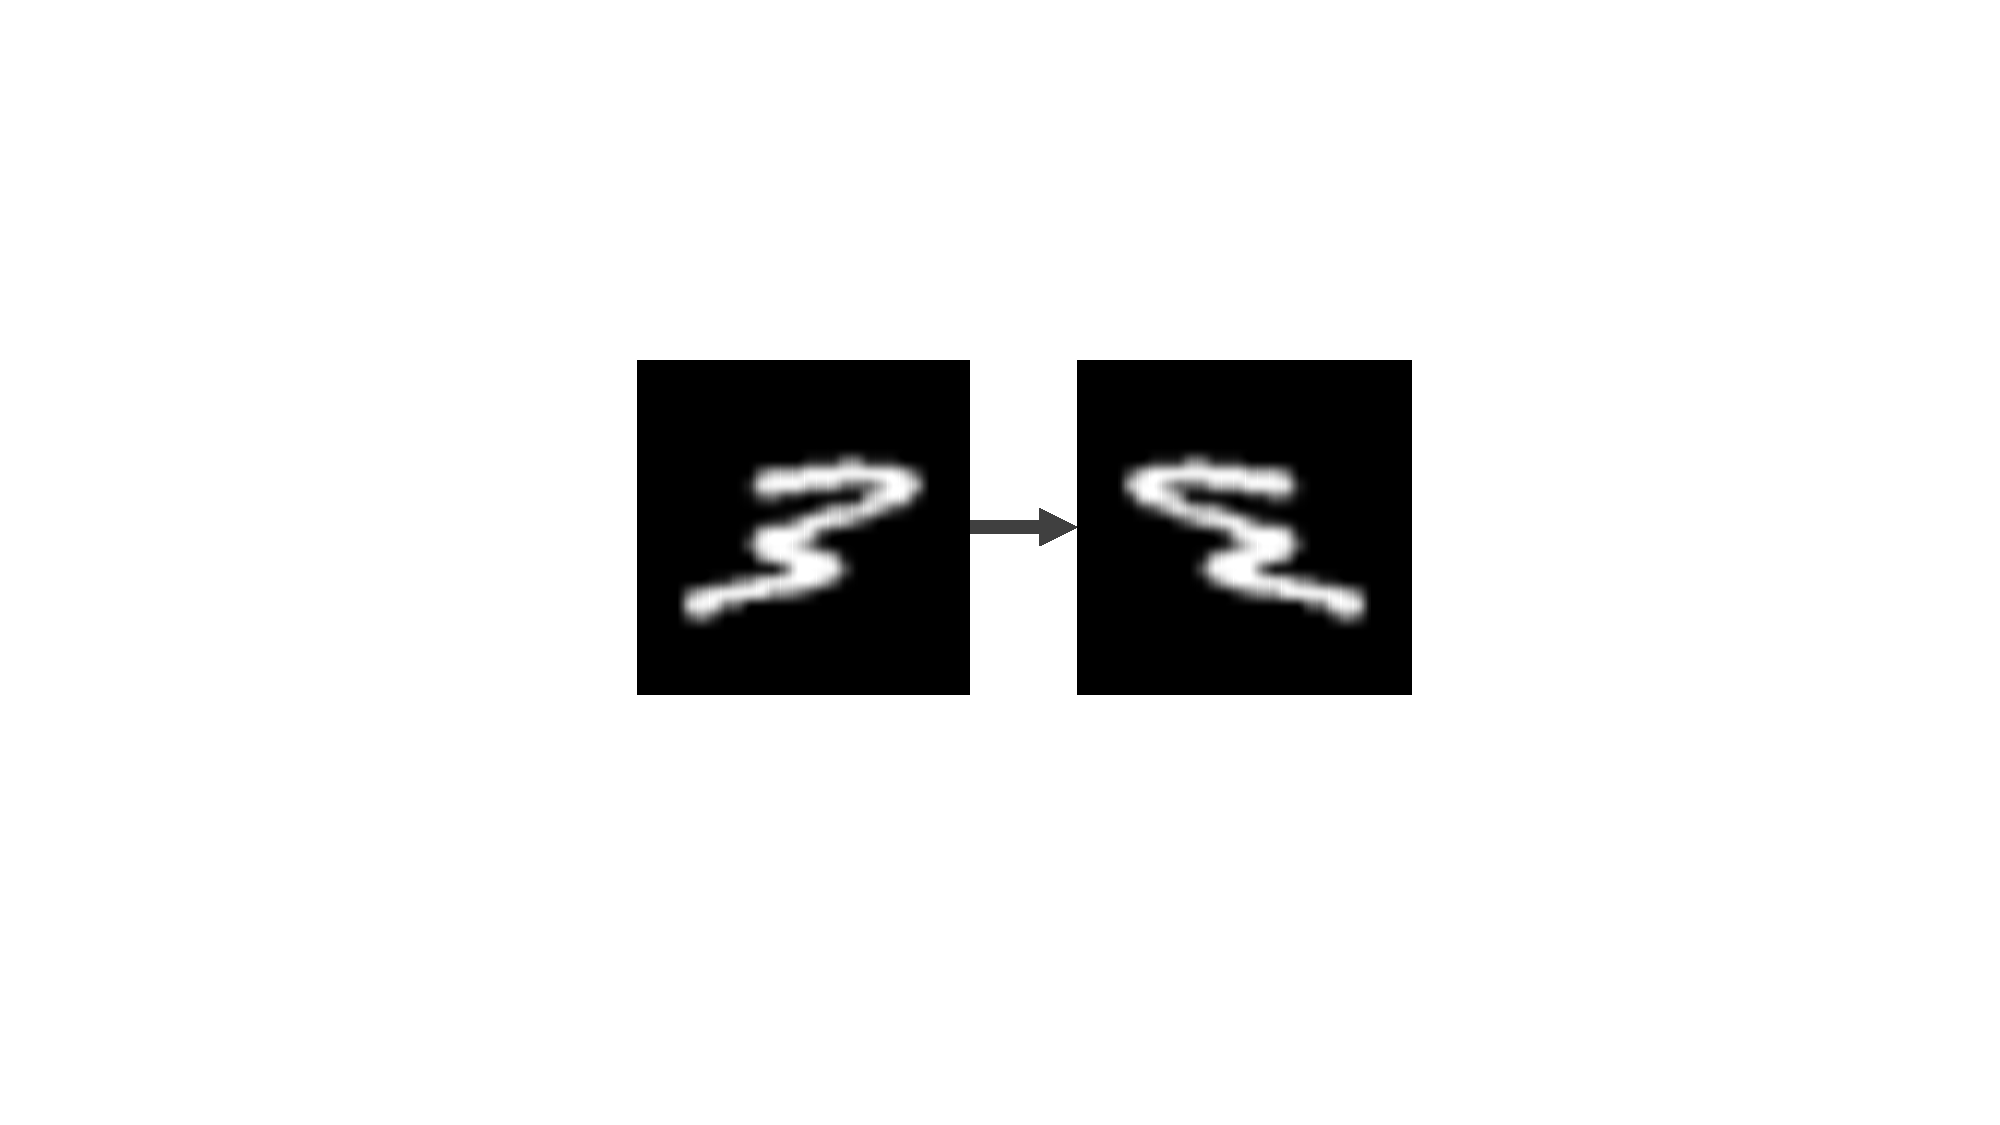
\includegraphics[width=1\linewidth]{lensed_hflip}
   \caption{}
   \label{flipping}
\end{subfigure}
\caption{(a) Horizontally flipped lensless image. (b) Shows what the data would look like if the network was using human-centric images as input.}\label{data_augmentations}
\end{figure}
%
\section{Results}
\subsection{Network Configurations}
We tested a lot of different configurations for our final network. Our earlier experimental networks actually achieved higher  accuracy than some of our later networks. Our later networks employed Leaky ReLU, PReLU, SELU activation functions and Alpha Dropout \cite{DBLP:journals/corr/HeZR015, Maas13rectifiernonlinearities, DBLP:journals/corr/KlambauerUMH17}. Leaky ReLU and PReLU are small variations on the conventional ReLU activation function. The margin between results for these variants compared to ReLU was roughly 2\% where ReLU scored higher than both variants. The problem we encountered using SELU and Alpha Dropout were using extra learnable parameters impacted our model's ability to learn. The highest accuracy we achieved using SELU and Alpha Dropout was 82\%.\par
Our final network was able achieve a 97\% accuracy and converged in fewer epochs than all of our experimental network configurations. Meaning, the final network was able to learn the necessary features quicker, in less time. While other gradient optimizers were tested such as Adam and Adagrad but we found that they did not converge accordingly \cite{DBLP:journals/corr/KingmaB14, Duchi:EECS-2010-24}. In all of our experiments, stochastic gradient decent with momentum was the best optimizer and allowed our network to converge to its global minimum.
\begin{figure}[!ht]
\centering
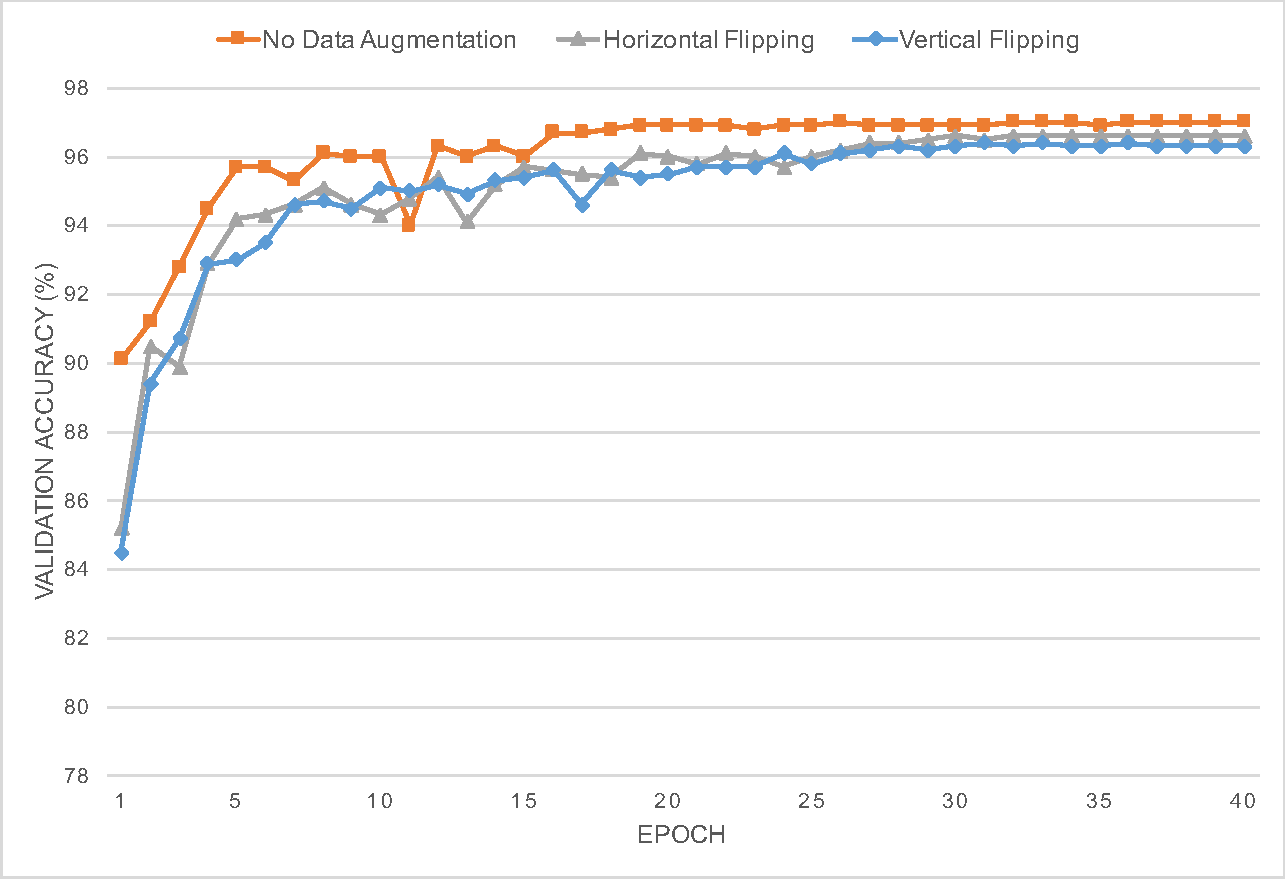
\includegraphics[width=.99\linewidth]{data_augmentation}
\caption{Comparison between results for no data augmentation, horizontal flipping and vertical flipping.}\label{augmentation_graph}
\end{figure}
%
\subsection{Experimental Data Augmentation}
Data augmentation is a widely used technique to artificially create more samples of data while training \cite{DBLP:journals/corr/WongGSM16}. We conducted a small test that horizontally and vertically flips the input data at a rate of 50\% shown in Figure \ref{data_augmentations}. Theoretically, creating more data samples should allow our network to learn more features and prevent overfitting in the network, but this idea has been applied only to human-centric images that we know of. In our tests, we found that the network performed slightly worse. Since these images are indecipherable by humans, we are not surprised that some data augmentation would hinder our network's ability to learn the necessary features to make accurate predictions. The differences between the results is minimal as shown in Figure \ref{augmentation_graph}.
%
\section{Conclusion}
In conclusion, we showed that Deep Learning is able to classify 10 handwritten digits with over 97\% accuracy using fully-lensless images. Since our camera is just an image sensor, it is easily incorporated into objects and can be applied in situations where human intervention is not required or desired (for privacy purposes, for example). Lensless cameras can be drastically lower in weight, which can enable new applications. When combined with Machine Learning, in general, such non-human cameras could enhance the decision making capabilities of artificial intelligence.
\section*{Funding}
 National Science Foundation (NSF) (1533611 and REU 1309041)
%
\bibliography{biblio}
\end{document}